\documentclass{../../slides-style}

\slidetitleext{Лекция 6: Тестирование и дефекты}{24.04.2025}{Тестирование и дефекты}

\begin{document}

    \begin{frame}[plain]
        \titlepage
    \end{frame}

    \section{Тестирование}

    \begin{frame}{Тестирование}
        \begin{outline}
            \1 Любая программа содержит ошибки
            \1 Если программа не содержит ошибок, их содержит алгоритм, который реализует эта программа
            \1 Если ни программа, ни алгоритм ошибок не содержат, такая программа даром никому не нужна
        \end{outline}
    \end{frame}

    \begin{frame}{Ошибки}
        \begin{outline}
            \1 Не несоответствие техническому заданию, а несоответствие ожиданиям
            \1 Процесс тестирования субъективен
        \end{outline}
    \end{frame}

    \begin{frame}{Баг}
        \begin{center}
            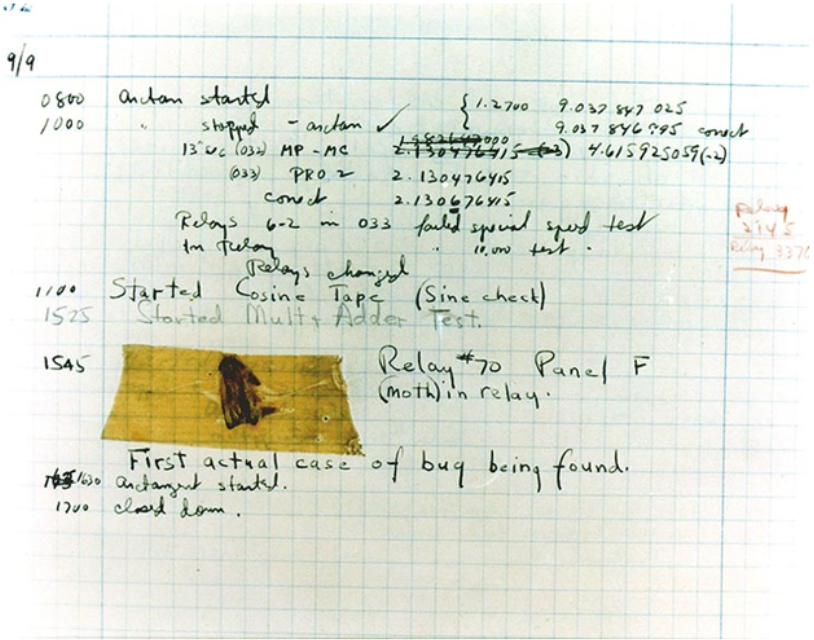
\includegraphics[width=0.7\textwidth]{bug.png}
            \attribution{https://education.nationalgeographic.org/resource/worlds-first-computer-bug/}
        \end{center}
    \end{frame}

    \begin{frame}{Цель тестирования}
        \begin{outline}
            \1 Тестирование~--- процесс поиска ошибок
                \2 Тест, не выявивший ошибку~--- впустую потраченное время
                    \3 Не совсем правда, есть регрессионные тесты
            \1 Тестирование не может доказать, что ошибок в программе нет
                \2 Субъективность ошибок
                \2 Огромное количество входных данных
                    \3 Программа, складывающая два целых числа~--- сотни лет на полный тест
                \2 Огромное количество путей исполнения
                    \3 1979 год, около 20 строк кода, сто триллионов путей исполнений
            \1 Формальная верификация
        \end{outline}
    \end{frame}

    \begin{frame}{Виды тестирования}
        \framesubtitle{Классификация по тому, что тестируется}
        \begin{outline}
            \1 Функциональное тестирование
            \1 Тестирование производительности
                \2 Нагрузочное
                \2 Стресс-тестирование
                \2 Тестирование стабильности
                \2 Тестирование конфигурации
            \1 Тестирование пользовательского интерфейса
            \1 Тестирование удобства использования
            \1 Тестирование безопасности
            \1 Тестирование локализации
            \1 Тестирование совместимости
        \end{outline}
    \end{frame}

    \begin{frame}{Виды тестирования}
        \framesubtitle{Классификация по масштабности тестирования}
        \begin{columns}
            \begin{column}{0.4\textwidth}
                \begin{outline}
                    \1 Модульное
                    \1 Интеграционное
                    \1 Системное
                        \2 В т.ч. тестирование пользовательского интерфейса
                \end{outline}
            \end{column}
            \begin{column}{0.6\textwidth}
                \begin{center}
                    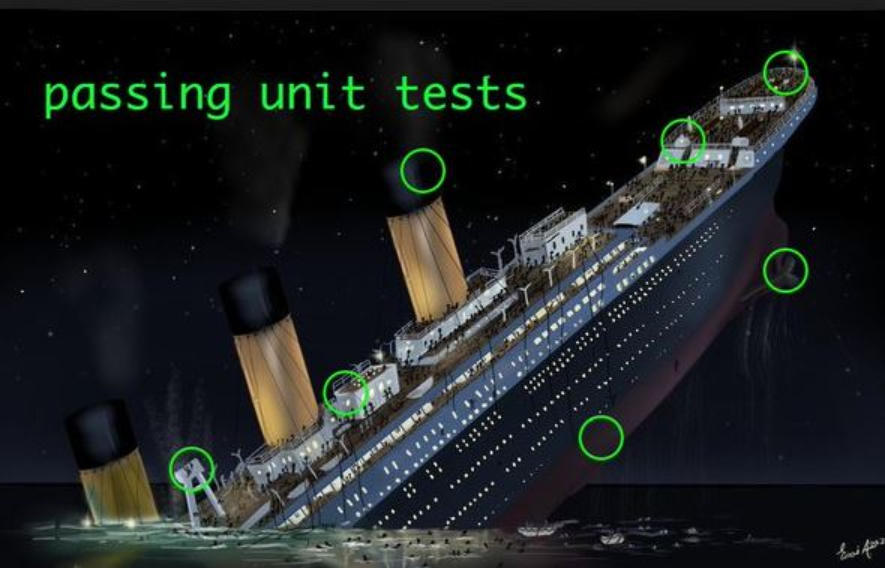
\includegraphics[width=\textwidth]{titanic.png}
                \end{center}
            \end{column}
        \end{columns}
    \end{frame}

    \begin{frame}{Виды тестирования}
        \framesubtitle{По этапу жизненного цикла}
        \begin{outline}
            \1 Смоук-тестирование
            \1 Регрессионное тестирование
            \1 Альфа-тестирование
            \1 Бета-тестирование
            \1 Релиз-кандидат
        \end{outline}
    \end{frame}

    \begin{frame}{Виды тестирования}
        \framesubtitle{По знанию о системе}
        \begin{outline}
            \1 Тестирование \enquote{чёрного ящика}
            \1 Тестирование \enquote{белого ящика}
            \1 Тестирование \enquote{серого ящика}
            \1 Исследовательское тестирование
        \end{outline}
    \end{frame}

    \section{Тестирование и жизненный цикл}

    \subsection{Тестирование требований}

    \begin{frame}{Тестирование требований}
        \begin{outline}
            \1 Однозначность
                \2 слова \enquote{обычно}, \enquote{как правило}, \enquote{иногда}, \enquote{необязательно} и т.п.
                \2 субъективные оценочные суждения: \enquote{удобно}, \enquote{быстро}, \enquote{гибко} и т.п.
            \1 Атомарность (без предлогов и/или)
            \1 Чёткий критерий приёмки (acceptance criteria)
            \1 Отсутствие избыточных и противоречивых требований
            \1 Мотивация каждой роли
            \1 Не предполагает конкретного способа реализации
        \end{outline}
    \end{frame}

    \begin{frame}{Критерии приёмки}
        \begin{outline}
            \1 Чёткие
            \1 Контекст-действие
            \1 Однозначно документирующие поведение системы
            \1 Добросовестные
        \end{outline}
    \end{frame}

    \subsection{Тестирование архитектуры}

    \begin{frame}{Тестирование архитектуры}
        \begin{outline}
            \1 Аккуратность декомпозиции
                \2 Dependency Inversion
                \2 Слои
                \2 Микросервисы
                    \3 Опасайтесь \enquote{микросервисного монолита}
            \1 Простота
            \1 Наблюдаемость
                \2 Возможность развернуть окружение
                \2 Быстрая обратная связь
                \2 Логирование
                    \3 Поддержанное инструментами, например ElasticSearch и Kibana
                \2 Трассируемость
                \2 Метрики
        \end{outline}
    \end{frame}

    \subsection{Тестирование и реализация}

    \begin{frame}{Тестирование и реализация}
        \framesubtitle{Пирамида тестирования}
        \begin{center}
            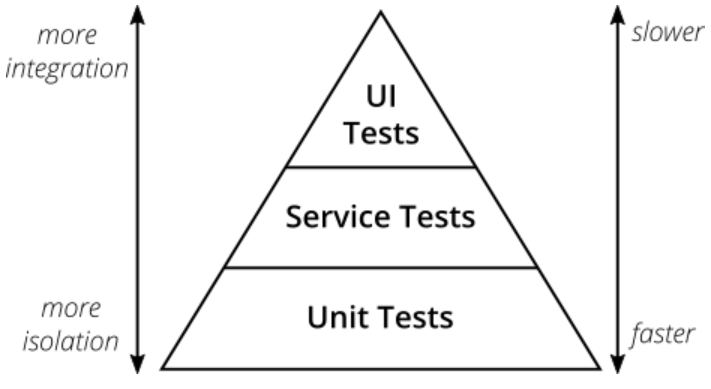
\includegraphics[width=0.7\textwidth]{testPyramid.png}
            \attribution{https://martinfowler.com/articles/practical-test-pyramid.html}
        \end{center}
    \end{frame}

    \begin{frame}{Тестовые сценарии, свойства}
        \begin{outline}
            \1 Идентификатор и название
            \1 Предварительные шаги
            \1 Тестовые шаги
                \2 Действие~--- ожидаемый результат
            \1 Итоговый ожидаемый результат
            \1 Шаги по восстановлению окружения
            \1 Конфигурация
            \1 Тэги
            \1 Зависимости
        \end{outline}
    \end{frame}

    \begin{frame}{Тесты, терминология}
        \begin{outline}
            \1 Сьюты
            \1 Проекты
            \1 Тестовые прогоны
                \2 Статус
                \2 Результаты по каждому шагу
            \1 Тест-планы
                \2 Отобранные тестовые сценарии
                \2 Календарные сроки
                \2 Ответственные
        \end{outline}
    \end{frame}

    \begin{frame}{Пример тестового сценария}
        \begin{center}
            \begin{tabu} {| X[0.6 l p] | X[1 l p] |}
                \tabucline-
                \everyrow{\tabucline-}
                \textbf{Что делаем}                             & \textbf{Что происходит}                                                            \\
                Вводим \textit{adder} и жмём на \textit{Enter}  & Экран мигает, внизу появляется знак вопроса                                        \\
                Нажимаем 2                                      & За знаком вопроса появляется цифра 2                                               \\
                Нажимаем \textit{Enter}                         & В следующей строке появляется знак вопроса                                         \\
                Нажимаем 3                                      & За вторым знаком вопроса появляется цифра 3                                        \\
                Нажимаем \textit{Enter}                         & В третьей строке появляется 5, несколькими строками ниже~--- ещё один знак вопроса
            \end{tabu}
        \end{center}
    \end{frame}

    \begin{frame}{Выявленные проблемы}
        \begin{outline}
            \1 Нет названия программы на экране, может, мы запустили не то
            \1 Нет никаких инструкций, пользователь без идей, что делать
            \1 Непонятно, как выйти
        \end{outline}
    \end{frame}

    \begin{frame}{Позитивный сценарий}
        \begin{scriptsize}
            \begin{center}
                \begin{tabu} {| X[2 l p] | X[2 l p] | X[7 l p] |}
                    \tabucline-
                    \everyrow{\tabucline-}
                    \textbf{Ввод}  & \textbf{Ожидаемый результат}  & \textbf{Замечания}                                                      \\
                    99 + 99        & 198                           & Пара наибольших допустимых чисел                                        \\
                    -99 + -99      & -198                          & Отрицательные числа, почему нет?                                        \\
                    99 + -14       & 85                            & Большое первое число может влиять на интерпретацию второго              \\
                    -38 + 99       & 61                            & Отрицательное плюс положительное                                        \\
                    56 + 99        & 155                           & Большое второе число может повлиять на интерпретацию первого            \\
                    9 + 9          & 18                            & Два наибольших числа из одной цифры                                     \\
                    0 + 0          & 0                             & Программы часто не работают на нулях                                    \\
                    0 + 23         & 23                            & 0~--- подозрительная штука, его надо проверить и как первое слагаемое,  \\
                    -78 + 0        & -78                           & и как второе
                \end{tabu}
            \end{center}
        \end{scriptsize}
    \end{frame}

    \begin{frame}{Негативные сценарии}
        \begin{scriptsize}
            \begin{center}
                \begin{tabu} {| X[2 l p] | X[7 l p] |}
                    \tabucline-
                    \everyrow{\tabucline-}
                    \textbf{Ввод}                   & \textbf{Замечания}                                                 \\
                    100 + 100                       & Поведение сразу за диапазоном допустимых значений                  \\
                    \textit{Enter} + \textit{Enter} & Что будет, если данные не вводить вообще                           \\
                    123456 + 0                      & Введём побольше цифр                                               \\
                    1.2 + 5                         & Вещественные числа, пользователь может решить, что так можно       \\
                    A + b                           & Недопустимые символы, что будет?                                   \\
                    Ctrl-A, Ctrl-D, F1, Esc         & Управляющие клавиши часто источник проблем в консольных программах \\
                \end{tabu}
            \end{center}
        \end{scriptsize}
    \end{frame}

    \begin{frame}{Ещё больше тестов!}
        \begin{outline}
            \1 Внутреннее хранение данных~--- двузначные числа могут хранить в \textbf{byte}
                \2 99 + 99, этот случай покрыли
            \1 Кодовая страница ввода: символы '/', '0', '9' и ':'
                \2 Программист может напутать со строгостью неравенства при проверке
                \2 Не надо вводить A + b, достаточно граничные символы
        \end{outline}
    \end{frame}

    \subsection{Инструменты тестирования}

    \begin{frame}[fragile]{Библиотеки модульного тестирования}
        \begin{outline}
            \1 JUnit со товарищи (NUnit, pytest и т.п.)
                \2 Инициализация SUT
                \2 Выполнение действия
                \2 Проверка результатов
            \1 Библиотеки матчеров: Hamcrest и т.п.
                \2 \mintinline{csharp}{Assert.That(f(), Is.EqualTo(1))}
                \2 NUnit умеет \enquote{из коробки}
            \1 Библиотеки тестирования, основанного на свойствах: QuickCheck, FsCheck
            \1 Библиотеки символьного исполнения
        \end{outline}
    \end{frame}

    \begin{frame}[fragile]{Библиотеки тестовых заглушек}
        \begin{outline}
            \1 Mockito, Moq и т.п.
        \end{outline}
        \begin{minted}{java}
LinkedList mockedList = mock(LinkedList.class);
// or even simpler with Mockito 4.10.0+
// LinkedList mockedList = mock();

// stubbing appears before the actual execution
when(mockedList.get(0)).thenReturn("first");

// the following prints "first"
System.out.println(mockedList.get(0));

// the following prints "null" because get(999) was not stubbed
System.out.println(mockedList.get(999));
        \end{minted}
    \end{frame}

    \begin{frame}{Тестирование интерфейсов}
        \begin{outline}
            \1 Пользовательские интерфейсы
                \2 Selenium: клик по координатам, запросы к DOM
                \2 White (Windows Accessibility API и т.п.)
            \1 Программные интерфейсы
                \2 Postman, Swagger вручную, модульные тесты с запросами
                \2 Фаззеры, сканеры безопасности
        \end{outline}
    \end{frame}

    \begin{frame}{Системы управления тестированием}
        \begin{outline}
            \1 Электронные таблицы, документы и т.п.
            \1 TestRail
            \1 Test IT, Xray, Kiwi TCMS, Sitechko
            \1 TestY
        \end{outline}
    \end{frame}

    \section{Отслеживание ошибок}

    \begin{frame}{Атрибуты отчёта об ошибке}
        \begin{outline}
            \1 Уникальный идентификатор
            \1 Заголовок
            \1 Описание дефекта
                \2 Контекст~--- версия, конфигурация и т.п.
                \2 Шаги воспроизведения~--- минимальны и воспроизводимы
                \2 Ожидаемый и полученный результаты
                \2 Дополнительная информация
            \1 Серьёзность (блокер, высокая, средняя, низкая, тривиальная)
            \1 Приоритет
            \1 Статус
            \1 Тип (ошибка, улучшение)
            \1 Автор, ответственный за исправление, ответственный за проверку
        \end{outline}
    \end{frame}

    \begin{frame}{Жизненный цикл ошибки}
        \begin{center}
            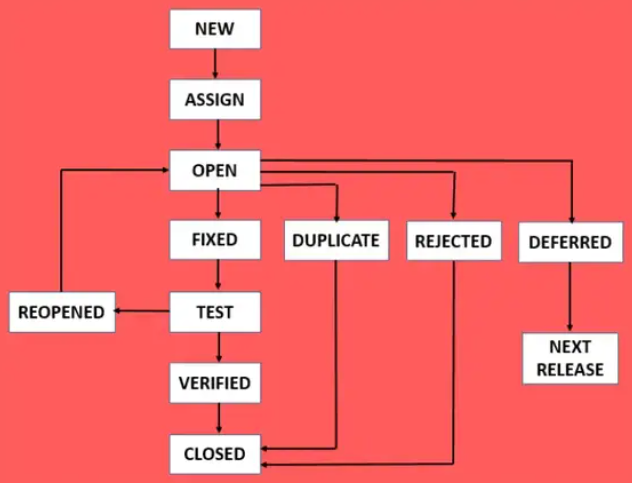
\includegraphics[width=0.6\textwidth]{bugLifecycle1.png}
            \attribution{https://www.softwaretestingmaterial.com/bug-life-cycle/}
        \end{center}
    \end{frame}

    \begin{frame}{Ещё пример}
        \begin{center}
            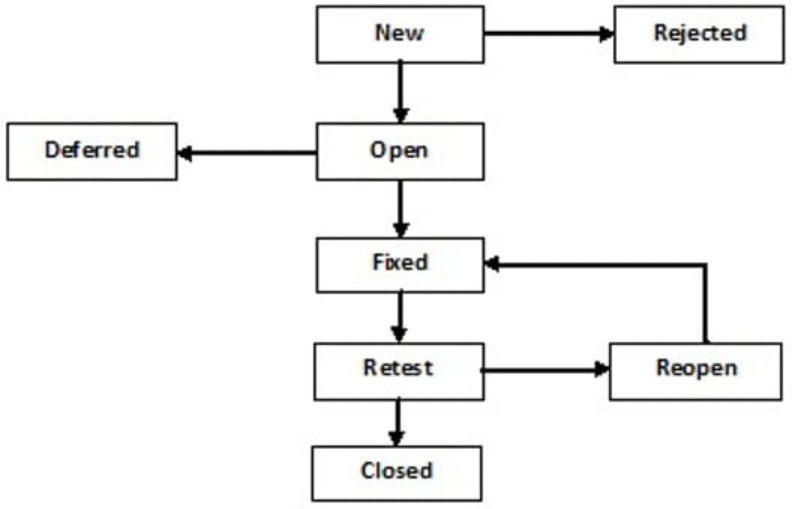
\includegraphics[width=0.6\textwidth]{bugLifecycle2.png}
            \attribution{https://www.softwaretestinghelp.com/bug-life-cycle/}
        \end{center}
    \end{frame}

    \begin{frame}{Системы отслеживания ошибок}
        \begin{outline}
            \1 Jira
            \1 GitHub Issues, Gitlab и т.п.
            \1 Yandex Tracker
            \1 Microsoft Team Foundation Server
            \1 Redmine
            \1 JetBrains Youtrack
            \1 Bugzilla
            \1 OpenProject
        \end{outline}
    \end{frame}

\end{document}